\documentclass[tikz,border=2pt]{standalone}
\usepackage{times}
\usepackage{amsmath}
\usepackage{fix-cm}
\usepackage{graphicx}
\usetikzlibrary{positioning,fit,calc,arrows.meta,backgrounds,shapes.misc,decorations.pathreplacing}

% Two accents; every other colour is a neutral or a tint of an accent.
\definecolor{rig}{HTML}{187F8C}
\definecolor{textcond}{HTML}{B96341}
\definecolor{ink}{HTML}{292D32}
\definecolor{muted}{HTML}{687078}
\definecolor{rule}{HTML}{B9BFC4}
\definecolor{wash}{HTML}{F4F5F6}
\newcommand{\labfont}{\fontsize{7.2}{8.3}\selectfont}
\newcommand{\smallfont}{\fontsize{7}{8}\selectfont}
\DeclareMathSizes{7.2}{7.2}{6.6}{6.6}
\DeclareMathSizes{7}{7}{6.6}{6.6}

% Both optional rasters fit a 0.9-in-wide footprint. Missing files leave
% labelled, empty placeholders; no external files are needed to compile.
\newcommand{\rigimage}{%
  \IfFileExists{rest_pose_skeleton.png}{%
    \includegraphics[width=.9in,height=38pt,keepaspectratio]{rest_pose_skeleton.png}%
  }{\parbox[c][38pt][c]{.9in}{\centering\smallfont\color{muted}%
    Rest-pose skeleton\\image placeholder}}}
\newcommand{\skinimage}{%
  \IfFileExists{skinned_character.png}{%
    \includegraphics[width=.9in,height=36pt,keepaspectratio]{skinned_character.png}%
  }{\parbox[c][36pt][c]{.9in}{\centering\smallfont\color{muted}%
    Skinned character\\image placeholder}}}

\begin{document}
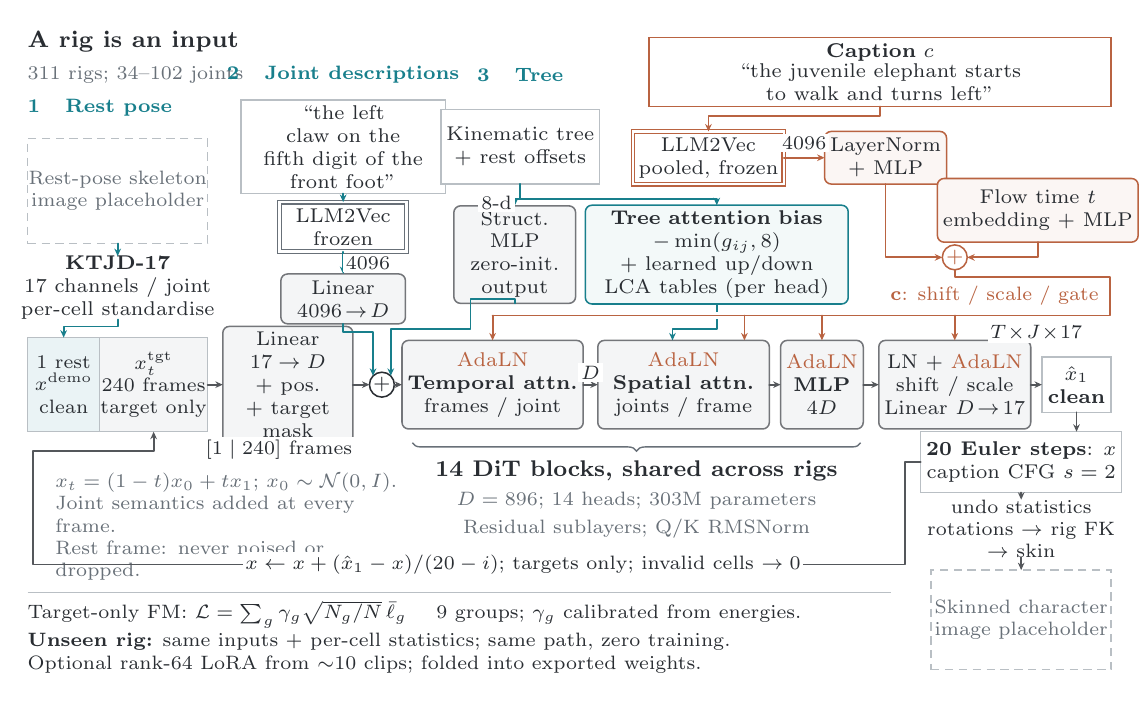
\begin{tikzpicture}[
  x=1pt,y=-1pt,
  font=\labfont,text=ink,
  every node/.style={align=center,inner sep=2pt,outer sep=0pt},
  data/.style={rectangle,draw=rule,fill=white,line width=.55pt},
  learned/.style={rectangle,rounded corners=2.4pt,draw=ink!65,
    fill=wash,line width=.55pt},
  frozen/.style={rectangle,draw=muted,double=white,double distance=1pt,
    fill=white,line width=.4pt},
  placeholder/.style={rectangle,draw=rule,densely dashed,
    line width=.55pt,inner sep=0pt,minimum width=.9in},
  sum/.style={circle,draw=ink,fill=white,line width=.55pt,
    minimum size=9pt,inner sep=0pt},
  a/.style={-{Stealth[length=2.7pt,width=2.4pt]},line width=.65pt,
    draw=ink!80,line cap=round,line join=round},
  wire/.style={line width=.65pt,line cap=round,line join=round},
  small/.style={font=\smallfont},
  tag/.style={font=\smallfont,fill=white,inner sep=1pt},
  title/.style={font=\fontsize{8.5}{9.5}\selectfont\bfseries,
    anchor=west,inner sep=0pt}
]
% 393.485 + 4 border pt = 5.5 in; 233 + 4 pt = 3.28 in.
\path[use as bounding box] (0,0) rectangle (393.485,233);

% Rig inputs: three independently readable routes.
\node[title] at (0,5) {A rig is an input};
\node[small,anchor=west,inner sep=0pt,text=muted] at (0,17)
  {311 rigs; 34--102 joints};
\node[small,anchor=west,text=rig,inner sep=0pt] at (0,29)
  {\textbf{1\quad Rest pose}};
\node[placeholder] (rest) at (32.52,59) {\rigimage};
\node[small,text=rig] at (114,17) {\textbf{2\quad Joint descriptions}};
\node[data,text width=70pt,minimum height=30pt] (descriptions) at (114,43)
  {``the left claw on the\\fifth digit of the\\front foot''};
\node[frozen,minimum width=46pt,minimum height=18pt] (jointenc) at (114,72)
  {LLM2Vec\\frozen};
\node[learned,minimum width=45pt,minimum height=18pt] (jointproj) at (114,98)
  {Linear\\$4096\!\to\!D$};
\draw[a,draw=rig] (descriptions.south) -- (jointenc.north);
\draw[a,draw=rig] (jointenc.south) -- node[tag,right] {$4096$} (jointproj.north);

\node[small,text=rig] at (178,17) {\textbf{3\quad Tree}};
\node[data,minimum width=45pt,minimum height=27pt] (tree) at (178,43)
  {Kinematic tree\\+ rest offsets};
\node[learned,text width=40pt,minimum height=23pt] (structure) at (176,82)
  {Struct. MLP\\zero-init.\\output};
\draw[a,draw=rig] (tree.south) -- (178,62) -| node[tag,pos=.75,left] {$8$-d} (structure.north);
\node[learned,draw=rig,fill=rig!5,text width=91pt,minimum height=32pt]
  (bias) at (249,82)
  {\textbf{Tree attention bias}\\$-\min(g_{ij},8)$\\+ learned up/down\\LCA tables (per head)};
\draw[a,draw=rig] (tree.south) -- (178,62) -- (249,62) -- (bias.north);

% Caption and flow time: a separate modulation route, never motion tokens.
\node[data,draw=textcond,text width=163pt,minimum height=25pt] (caption) at (308,16)
  {\textbf{Caption $c$}\\[-1pt]
   ``the juvenile elephant starts to walk and turns left''};
\node[frozen,draw=textcond,minimum width=46pt,minimum height=19pt] (captionenc) at (246,47)
  {LLM2Vec\\pooled, frozen};
\node[learned,draw=textcond,fill=textcond!6,minimum width=44pt,minimum height=19pt]
  (captionmlp) at (310,47) {LayerNorm\\+ MLP};
\node[learned,draw=textcond,fill=textcond!6,minimum width=50pt,minimum height=23pt]
  (timemlp) at (365,66) {Flow time $t$\\embedding + MLP};
\node[sum,draw=textcond,text=textcond] (condsum) at (335,83) {$+$};
\draw[a,draw=textcond] (caption.south) -- (308,32) -- (246,32) -- (captionenc.north);
\draw[a,draw=textcond] (captionenc.east) -- node[tag,above=2pt] {$4096$} (captionmlp.west);
\draw[a,draw=textcond] (captionmlp.south) |- (condsum.west);
\draw[a,draw=textcond] (timemlp.south) |- (condsum.east);

% Rest-pose conversion and the explicit [one clean | 240 target] layout.
\node[inner sep=0pt] (representation) at (32.52,94)
  {\textbf{KTJD-17}\\17 channels / joint\\per-cell standardise};
\draw[a,draw=rig] (rest.south) -- (representation.north);
\draw[data,fill=rig!9] (0,112) rectangle (26,146);
\draw[data,fill=wash] (26,112) rectangle (65.04,146);
\node[small,inner sep=0pt] at (13,129) {1 rest\\$x^{\rm demo}$\\clean};
\node[small,inner sep=0pt] at (45.52,129) {$x_t^{\rm tgt}$\\240 frames\\target only};
\coordinate (targetbottom) at (45.52,146);
\coordinate (seqeast) at (65.04,129);
\draw[a,draw=rig] (representation.south) -- (32.52,108) -- (13,108) -- (13,112);
\node[learned,text width=43pt,minimum height=34pt] (embed) at (94,129)
  {Linear\\$17\!\to\!D$\\+ pos.\\+ target mask};
% "pos." = learned temporal + learned joint-slot positions.
% The learned mask token is added only to target frames.
\node[sum] (tokensum) at (128,129) {$+$};
\draw[a] (seqeast) -- node[tag,below=19pt,xshift=23pt] {$[1\mid240]$ frames} (embed.west);
\draw[a] (embed.east) -- (tokensum.west);
\draw[a,draw=rig] (jointproj.south) -- (114,110) -- (124.8,110) -- (124.8,125.8);
\draw[a,draw=rig] (structure.south) -- (176,98) -- (160,98) -- (160,109)
  -- (131.2,109) -- (131.2,125.8);

% Expanded repeated transformer block. All three modules are residual.
\node[learned,minimum width=58pt,minimum height=32pt] (temporal) at (168,129)
  {\textcolor{textcond}{AdaLN}\\\textbf{Temporal attn.}\\frames / joint};
\node[learned,minimum width=62pt,minimum height=32pt] (spatial) at (237,129)
  {\textcolor{textcond}{AdaLN}\\\textbf{Spatial attn.}\\joints / frame};
\node[learned,minimum width=28pt,minimum height=32pt] (mlp) at (287,129)
  {\textcolor{textcond}{AdaLN}\\\textbf{MLP}\\$4D$};
\node[learned,minimum width=47pt,minimum height=32pt] (head) at (335,129)
  {LN + \textcolor{textcond}{AdaLN}\\shift / scale\\Linear $D\!\to\!17$};
\node[data,minimum width=25pt,minimum height=20pt] (clean) at (379,129)
  {$\hat{x}_1$\\\textbf{clean}};
\draw[a] (tokensum.east) -- (temporal.west);
\draw[a] (temporal.east) -- node[tag,above=1pt] {$D$} (spatial.west);
\draw[a] (spatial.east) -- (mlp.west);
\draw[a] (mlp.east) -- (head.west);
\draw[a] (head.east) -- node[tag,above=15pt] {$T\!\times\!J\!\times\!17$} (clean.west);
% The tree bias enters spatial attention directly. One wire crossover is
% deliberately drawn without a junction; the white casing separates it.
\draw[a,draw=rig] (bias.south) -- (249,109) -- (233,109) -- (233,113);
\draw[wire,draw=white,line width=2.8pt] (168,104) -- (335,104);
\draw[wire,draw=textcond] (condsum.south) -- (335,90) -- (391,90) -- (391,104) -- (168,104);
\node[tag,text=textcond,anchor=east] at (388,97) {$\mathbf c$: shift / scale / gate};
\foreach \xx in {168,259,287,335}{
  \draw[a,draw=textcond] (\xx,104) -- (\xx,113);
}
\draw[decorate,decoration={brace,amplitude=3pt},draw=muted,line width=.5pt]
  (301,150) -- (139,150);
\node[font=\fontsize{8.2}{9}\selectfont\bfseries] at (220,160)
  {14 DiT blocks, shared across rigs};
\node[small,text=muted] at (220,171) {$D=896$; 14 heads; 303M parameters};
\node[small,text=muted] at (220,181) {Residual sublayers; Q/K RMSNorm};
\node[small,align=left,anchor=north west,inner sep=0pt,text width=125pt,text=muted] at (10,161)
  {$x_t=(1-t)x_0+t x_1$; $x_0\sim\mathcal N(0,I)$.\\Joint semantics added at every frame.\\Rest frame: never noised or dropped.};

% Sampling and rig-specific decoding; the loop returns only to targets.
\node[data,minimum width=65pt,minimum height=22pt] (euler) at (359,157)
  {\textbf{20 Euler steps}: $x$\\caption CFG $s=2$};
\draw[a] (clean.south) -- (clean.south |- euler.north);
% This data box contains the evolving target state x. Caption CFG uses
% two network evaluations per Euler step; the rest prompt stays fixed.
\node[inner sep=0pt,small] (decode) at (359,181)
  {undo statistics\\rotations $\to$ rig FK\\$\to$ skin};
% Predicted position channels can also be decoded directly. This branch
% shows the rotation/FK route used to produce the skinned raster.
\draw[a] (euler.south) -- (decode.north);
\node[placeholder] (character) at (359,214) {\skinimage};
\draw[a] (decode.south) -- (character.north);
\draw[a] (euler.west) -- (317,157) -- (317,194) -- (2,194) -- (2,153)
  -- (45.52,153) -- (targetbottom);
\node[tag,small] at (179,194)
  {$x\leftarrow x+(\hat{x}_1-x)/(20-i)$; targets only; invalid cells $\to0$};

% Training is a quiet footnote, not a fourth pipeline region.
\draw[draw=rule,line width=.4pt] (0,204) -- (312,204);
\node[small,anchor=west,inner sep=0pt] at (0,212)
  {Target-only FM: $\mathcal L=\sum_g\gamma_g\sqrt{N_g/N}\,\bar\ell_g$
   \quad 9 groups; $\gamma_g$ calibrated from energies.};
\node[small,anchor=west,inner sep=0pt] at (0,222)
  {\textbf{Unseen rig:} same inputs + per-cell statistics; same path, zero training.};
\node[small,anchor=west,inner sep=0pt] at (0,230)
  {Optional rank-64 LoRA from $\sim$10 clips; folded into exported weights.};
\end{tikzpicture}
\end{document}
